\documentclass[11pt, letterpaper]{article}

\usepackage[utf8]{inputenc}
\usepackage{epsfig, url}
\usepackage{epstopdf}
\usepackage{tabularx}
\usepackage{graphicx}
\usepackage{datetime}
\usepackage{multirow}
\usepackage{float}
%\usepackage{wrapfig}
\usepackage{amsmath}
\usepackage{amssymb}
\usepackage{geometry} 
\geometry{a4paper}              

\usepackage{titling}
\setlength{\evensidemargin}{0in}
\setlength{\oddsidemargin}{0in}
\setlength{\textwidth}{6.5in}
\setlength{\textheight}{9.0in}
\setlength{\topmargin}{0in}
\setlength{\headheight}{0in}
\setlength{\headsep}{0in}
\setlength{\itemsep}{-\parsep}
\usepackage{amsthm}
\begin{document}

\title{\large Course CS-451: Computational Intelligence\\[0.5cm]
        \bf\Large Assignment 01 - Report}
\author{\large Ali Hamza (ah05084) \\ Haris Karim Ladhani (hl04349) \\ Synclair Samson (ss05901))}
\date{\today}
\makeatletter
    \begin{titlepage}
        \begin{center}
        \vbox{}\vspace{5cm}
            {\@title }\\[3cm] 
            {\@author}\\
            %{Instructor: \bf instructor name}\\
            \vfill 
\includegraphics[scale=0.5]{images/logo.png}\\[1cm]
            {\@date}
        \end{center}
    \end{titlepage}
\makeatother

\newpage

\tableofcontents

\newpage

\section{Genetic Algorithm Implementation}
\subsection{Parameters}
We have chosen default parameters as a control to run our tests between what selection schemes give the best results.
\begin{itemize}
    \item Population Size: $30$
    \item OffSpring per Generation: $10$
    \item Number of Generations: $100$
    \item Mutation rate: $0.4$
    \item Number of Iterations: $40$ 
\end{itemize}
\subsection{Crossover}
The generic crossover function works as follows:
\begin{enumerate}
    \item Select two random individuals from the selected parents
    \item Select the first half the first individual and the second half of the second individual to create a child Chromosome
    \item Select the first half of the second individual and the second half of the first individual to create a child Chromosome
    \item Mutate the child Chromosomes
    \item Append the child Chromosomes to the new population
\end{enumerate}
This function slightly changes in TSP as we cannot have repeated genes in a chromosome. A random crossover point is chosen for the first individual and then the remainder of the second individual is added to the child chromosome. The process is repeated with the second individual and the first individuals flipped. The child chromosomes are then mutated and appended to the new population.
\subsection{Mutation}
The mutation function is quite simplistic where a chromosome is taken permutated on the basis of the mutation rate.
\subsection{Chromosome Representations and Fitness Function}
\subsubsection{Travelling Salesman Problem (TSP)}
The Travelling Salesman Problem (TSP) is a problem in which a salesman has to visit a number of cities and return to the starting city. The salesman has to visit each city exactly once and return to the starting city. The distance between two cities is the Euclidean distance. 

To make implementation easier we removed the last restriction of the returning to the same city. The cities are represented as a list of coordinates, where each coordinate is a tuple of the form (x,y). 

Each chromosome is represented as an ordered array of cities. The population was initialized by simply taking a random permutation of the initial list of cities. The following is a representation of a chromosome: 
$$permutation([(x_1, y_1), (x_2,y_2), \dots, (x_n, y_n)])$$

The Fitness function is the total distance of the chromosome that was calculated by summing the distances between each city in the chromosome. The distance between two cities is then calculated as the Euclidean distance between two consecutive cities. This computation is slightly expensive as it involves a nested for loop of a time complexity of $O(n^2)$. The fitness of each chromosome can be mathematically represented as follows:
$$\sum_{i=1}^{n-1} \sqrt{(x_i - x_{i+1})^2 + (y_i - y_{i+1})^2}$$
It is obvious that this is a minimization problem therefore the smaller the fitness value the better the solution.

\subsubsection{Graph Coloring}
The Graph Coloring problem is a problem in which a graph is colored with a number of colors such that no two adjacent vertices are colored with the same color. The graph is represented as a list of edges, where each edge is a tuple of the form (u,v). The maximum coloring of a graph will be the number of nodes in the graph.

Therefore, the chromosome is represented as an array of colors represented as integers ranging from 1 to $n$, where $n$ is the number of nodes in the graph. The population was initialized by simply taking random integers between 1 and $n$ for each edge. The following is a representation of a chromosome:
% $$random(1,n), random(1,n), \dots, random(1,n)$$

The fitness is then the number of color violations present in a solution. The number of color violations is calculated by counting the number of edges that are adjacent to two vertices that have the same color. This computation is slightly expensive as it involves a nested for loop of a time complexity of $O(n^2)$. The fitness of each chromosome can be mathematically represented as follows:
$$\sum_{i=1}^{n-1} \left\{ \left\{ \begin{array}{ll} 1 & \text{if} \; \text{color}(i) = \text{color}(i+1) \\ 0 & \text{otherwise} \end{array} \right. \right\}$$

Of course, there is a limitation within this fitness function which is that it does not account for a minimum unique coloring. This adds a level of complexity to the problem which was not implemented for the scope of this assignment. It is obvious that the lower the number of edge violations the better the solution, therefore this is a minimization problem.
\subsubsection{Knapsack}
The Knapsack problem is a problem in which a knapsack is filled with a number of items such that the total weight of the items is less than or equal to the capacity of the knapsack. The items are represented as a list of tuples of the form (weight, value). The knapsack is represented as a list of tuples of the form (weight, value). 

The chromosome is represented as an array of $1$'s and $0$'s siginfying whether the item at that particual index was added to the knapsack or not. Therefore, a chromosome looks as follows:
$$\[randomint(0,1), randomint(0,1), \dots, randomint(0,1)\]$$

The fitness is then the total value of the items in the knapsack. The total value is calculated by summing the values of the items in the knapsack. The fitness of each chromosome can be mathematically represented as follows:

$$\sum_{i=0}^{n} \left\{ \left\{ \begin{array}{ll} value(i) & \text{if} \; \text{item}(i) = 1 \\ 0 & \text{otherwise} \end{array} \right. \right\}$$

The limitation of this fitness function is that it does not account for a high weight knapsack, another parameter that could be considered is the total weight of the knapsack when looking at the fitness of the knapsack - then the fitness function could be the $\frac{total_value}{total_weight}$. This adds a level of complexity to the problem which was not implemented for the scope of this assignment therefore we did not implement it. It is obvious that the higher the total value of the items in the knapsack the better the solution, therefore this is a maximization problem.
\section{Statistics and Analysis}

\subsection{Travelling Salesman Problem(TSP)}

\subsection{Results} 
\subsubsection {FPS and Random}
\begin{figure}[H]
    \centering
    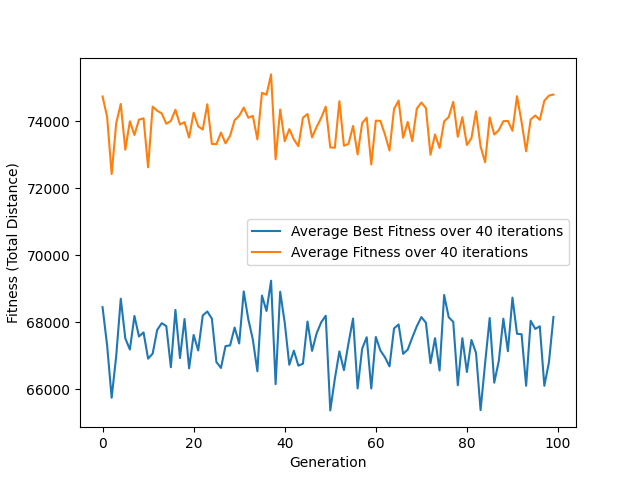
\includegraphics[scale = 0.6]{images/tsp_fp_rd.png}
    \caption {TSP - FPS \& Random}
    \label {fig:tpsFR}
\end{figure}
\subsubsection {RBS and Truncation}
\begin{figure}[h]
    \centering
    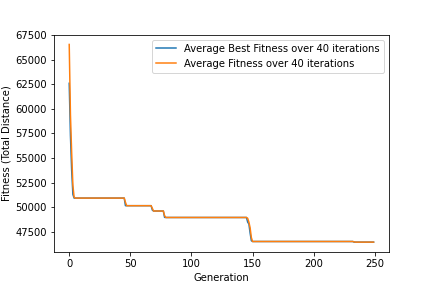
\includegraphics[scale = 0.6]{images/tsp_rb_tr.png}
    \caption {TSP - RBS \& Truncation}
    \label {fig:tpsBT}
\end{figure}

\subsubsection {Truncation and Truncation}

\begin{figure}[H]
    \centering
    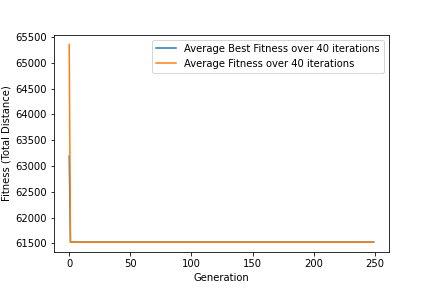
\includegraphics[scale = 0.6]{images/tsp_tr_tr.png}
    \caption {TSP - Truncation \& Truncation}
    \label {fig:tpsTT}
\end{figure}
\subsubsection {Random and Random}
\begin{figure}[H]
    \centering
    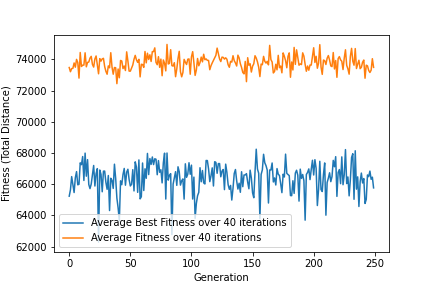
\includegraphics[scale = 0.6]{images/tsp_rd_rd.png}
    \caption {TSP - Random \& Random}
    \label {fig:tpsRR}
\end{figure}
\subsubsection {FPS and Truncation}
\begin{figure}[H]
    \centering
    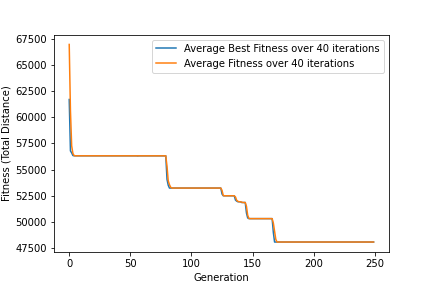
\includegraphics[scale = 0.6]{images/tsp_fp_tr.png}
    \caption {TSP - FPS \& Truncation}
    \label {fig:tpsFT}
\end{figure}
\subsubsection {Random and FPS}
\begin{figure}[H]
    \centering
    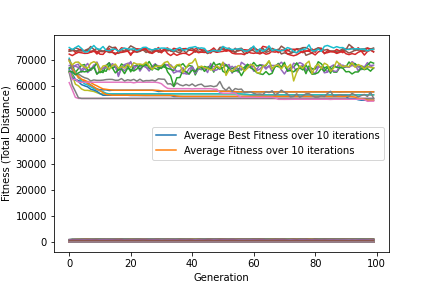
\includegraphics[scale = 0.6]{images/tsp_rd_fp.png}
    \caption {TSP - Random \& FPS}
    \label {fig:tpsRB}
\end{figure}

\subsubsection {Random and Truncation}
\begin{figure}[H]
    \centering
    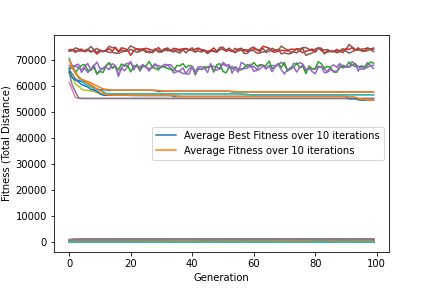
\includegraphics[scale = 0.6]{images/tsp_rd_tr.png}
    \caption {TSP - Random \& Truncation}
    \label {fig:tpsRT}
\end{figure}
\subsubsection {Truncation and RBS}
\begin{figure}[H]
    \centering
    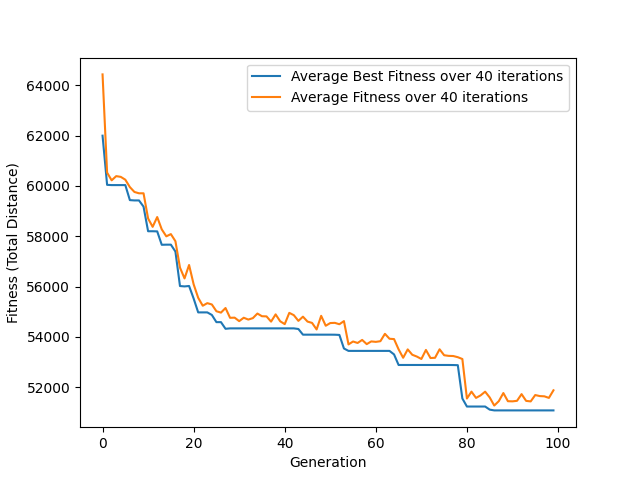
\includegraphics[scale = 0.6]{images/tsp_tr_rb.png}
    \caption {TSP - Truncation \& RBS}
    \label {fig:tpsTR}
\end{figure}
\subsubsection {RBS and Random}
\begin{figure}[H]
    \centering
    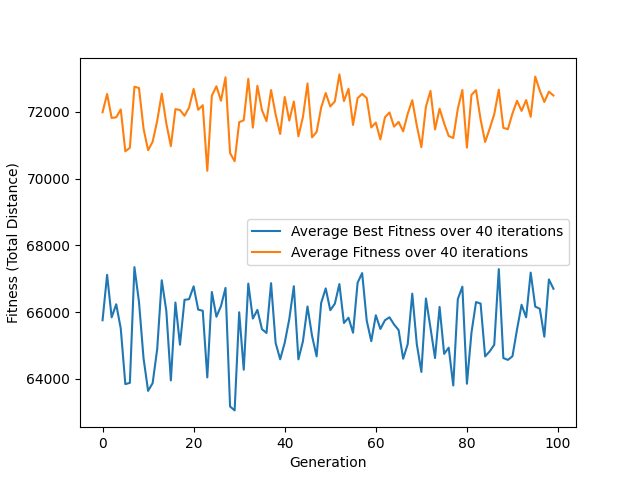
\includegraphics[scale = 0.6]{images/tsp_rb_rd.png}
    \caption {TSP - RBS \& Random}
    \label {fig:tpsRbR}
\end{figure}
\subsection {Overall Analysis}

\newpage

\section{Knapsack Problem}

\subsection{Results} 
\subsubsection {FPS and Random}
\begin{figure}[H]
    \centering
    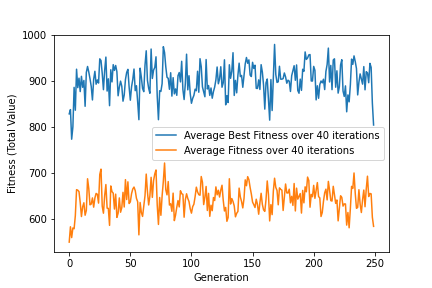
\includegraphics[scale = 0.6]{images/knapsack_fp_rd.png}
    \caption {Knapsack - FPS \& Random}
    \label {fig:kpFR}
\end{figure}
\subsubsection {RBS and Truncation}
\begin{figure}[h]
    \centering
    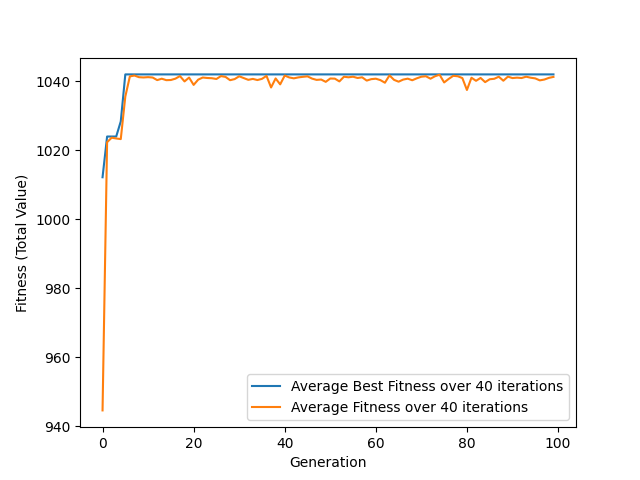
\includegraphics[scale = 0.6]{images/knapsack_rb_tr.png}
    \caption {Knapsack - RBS \& Truncation}
    \label {fig:kpBT}
\end{figure}

\subsubsection {Truncation and Truncation}
\begin{figure}[H]
    \centering
    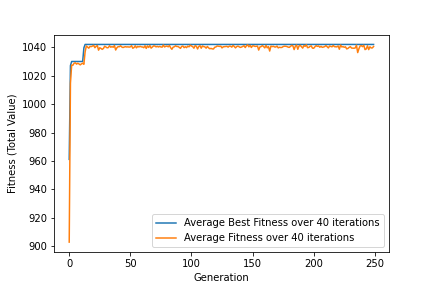
\includegraphics[scale = 0.6]{images/knapsack_tr_tr.png}
    \caption {Knapsack - Truncation \& Truncation}
    \label {fig:kpTT}
\end{figure}

\subsubsection {Random and Random}
\begin{figure}[H]
    \centering
    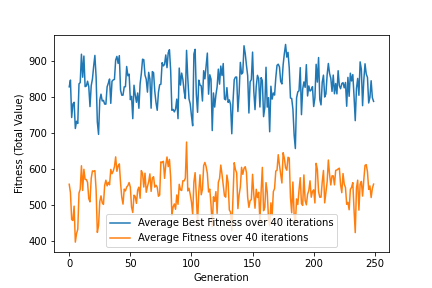
\includegraphics[scale = 0.6]{images/knapsack_rd_rd.png}
    \caption {Knapsack - Random \& Random}
    \label {fig:kpRR}
\end{figure}

\subsubsection {FPS and Truncation}
\begin{figure}[H]
    \centering
    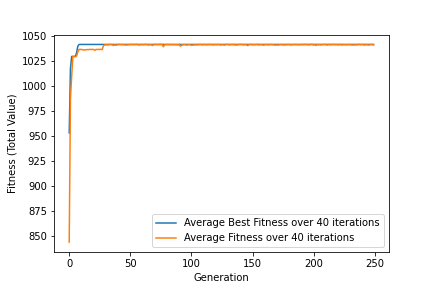
\includegraphics[scale = 0.6]{images/knapsack_fp_tr.png}
    \caption {Knapsack - FPS \& Truncation}
    \label {fig:kpFT}
\end{figure}

\subsubsection {Random and FPS}
\begin{figure}[H]
    \centering
    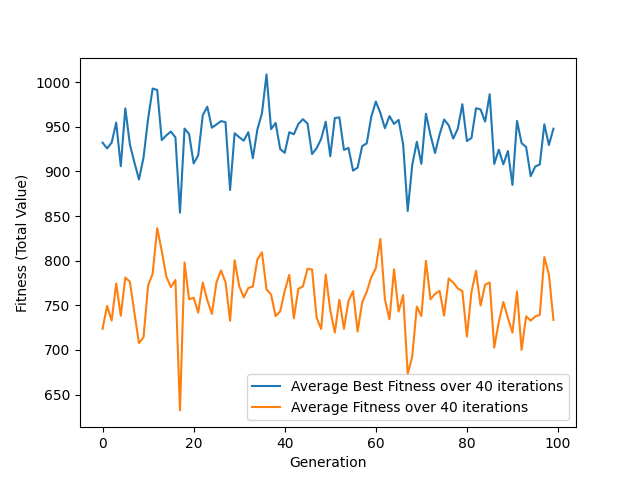
\includegraphics[scale = 0.6]{images/knapsack_rd_fp.png}
    \caption {Knapsack - Random \& FPS}
    \label {fig:kpRB}
\end{figure}

\subsubsection {Random and Truncation}
\begin{figure}[H]
    \centering
    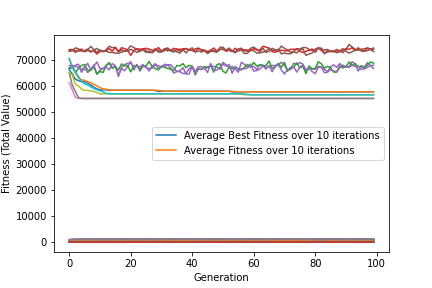
\includegraphics[scale = 0.6]{images/knapsack_rd_tr.png}
    \caption {Knapsack - Random \& Truncation}
    \label {fig:kpRT}
\end{figure}

\subsubsection {Truncation and RBS}
\begin{figure}[H]
    \centering
    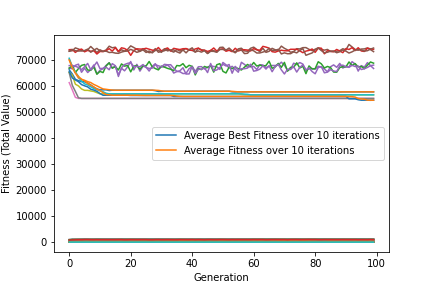
\includegraphics[scale = 0.6]{images/knapsack_tr_rb.png}
    \caption {Knapsack - Truncation \& RBS}
    \label {fig:kpTR}
\end{figure}

\subsubsection {RBS and Random}
\begin{figure}[H]
    \centering
    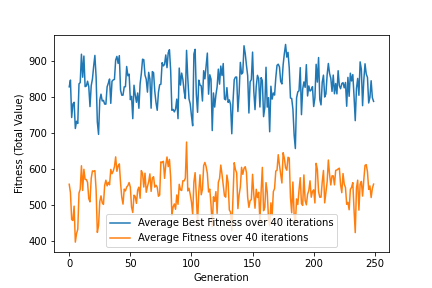
\includegraphics[scale = 0.6]{images/knapsack_rd_rd.png}
    \caption {Knapsack - RBS \& Random}
    \label {fig:kpRbR}
\end{figure}

\subsection {Overall Analysis}

\newpage

\section{Graph Coloring}
\subsection {Results} 
\subsubsection {FPS and Random}
\begin{figure}[H]
    \centering
    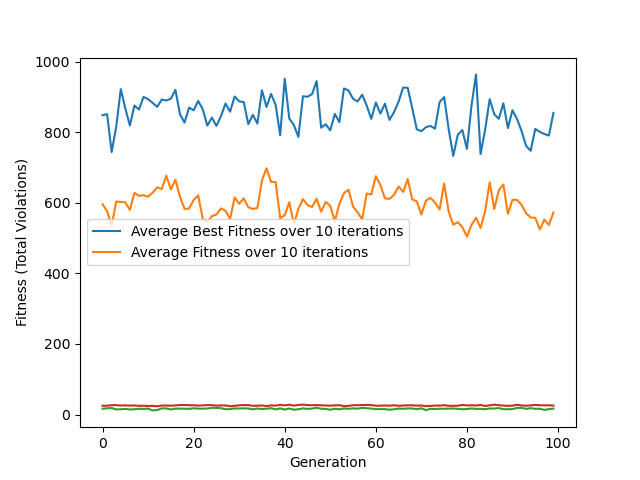
\includegraphics[scale = 0.6]{images/graphcoloring_fp_rd.png}
    \caption {Graph Coloring - FPS \& Random}
    \label {fig:gcFR}
\end{figure}
\subsubsection {RBS and Truncation}
\begin{figure}[h]
    \centering
    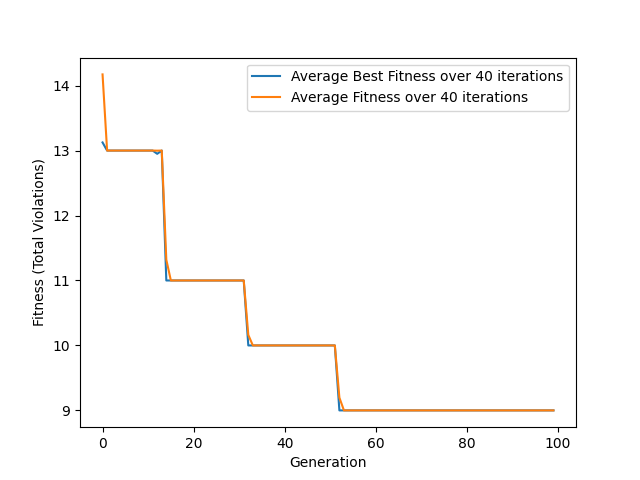
\includegraphics[scale = 0.6]{images/graphcoloring_rb_tr.png}
    \caption {Graph Coloring - RBS \& Truncation}
    \label {fig:gcBT}
\end{figure}

\subsubsection {Truncation and Truncation}
\begin{figure}[H]
    \centering
    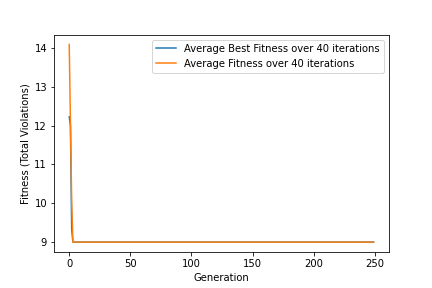
\includegraphics[scale = 0.6]{images/graphcoloring_tr_tr.png}
    \caption {Graph Coloring - Truncation \& Truncation}
    \label {fig:gcTT}
\end{figure}

\subsubsection {Random and Random}
\begin{figure}[H]
    \centering
    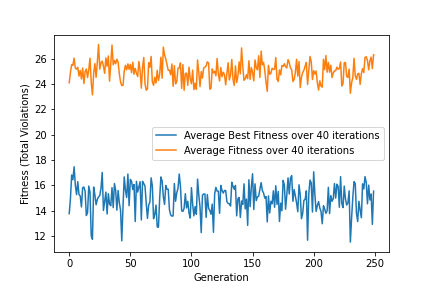
\includegraphics[scale = 0.6]{images/graphcoloring_rd_rd.png}
    \caption {Graph Coloring - Random \& Random}
    \label {fig:gcRR}
\end{figure}

\subsubsection {FPS and Truncation}
\begin{figure}[H]
    \centering
    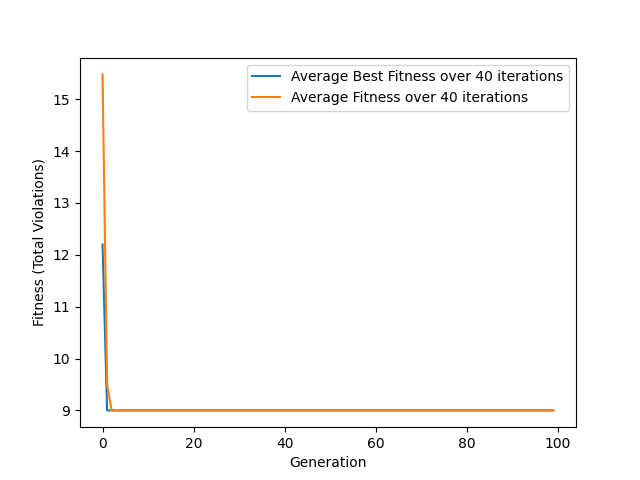
\includegraphics[scale = 0.6]{images/graphcoloring_fp_tr.png}
    \caption {Graph Coloring - FPS \& Truncation}
    \label {fig:gcFT}
\end{figure}

\subsubsection {Random and FPS}
\begin{figure}[H]
    \centering
    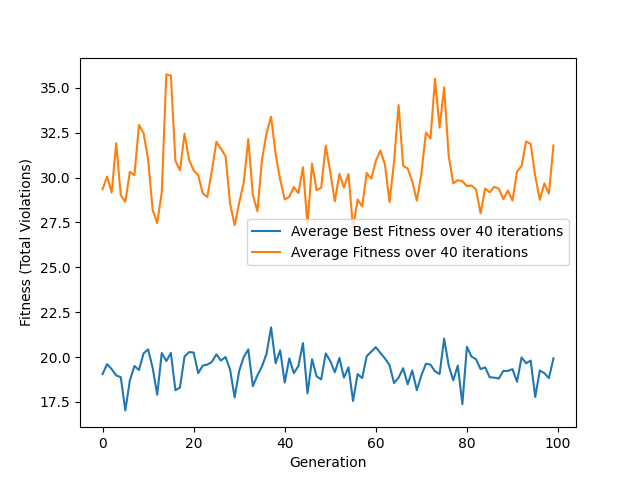
\includegraphics[scale = 0.6]{images/graphcoloring_rd_fp.png}
    \caption {Graph Coloring - Random \& FPS}
    \label {fig:gcRB}
\end{figure}

\subsubsection {Random and Truncation}
\begin{figure}[H]
    \centering
    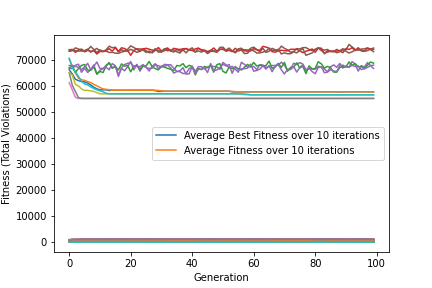
\includegraphics[scale = 0.6]{images/graphcoloring_rd_tr.png}
    \caption {Graph Coloring - Random \& Truncation}
    \label {fig:gcRT}
\end{figure}

\subsubsection {Truncation and RBS}
\begin{figure}[H]
    \centering
    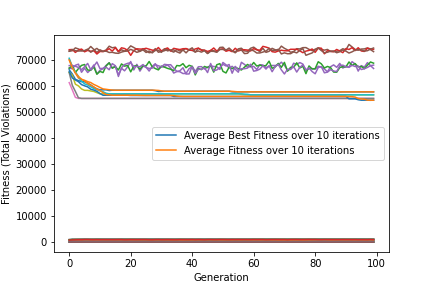
\includegraphics[scale = 0.6]{images/graphcoloring_tr_rb.png}
    \caption {Graph Coloring - Truncation \& RBS}
    \label {fig:gcTR}
\end{figure}

\subsubsection {RBS and Random}
\begin{figure}[H]
    \centering
    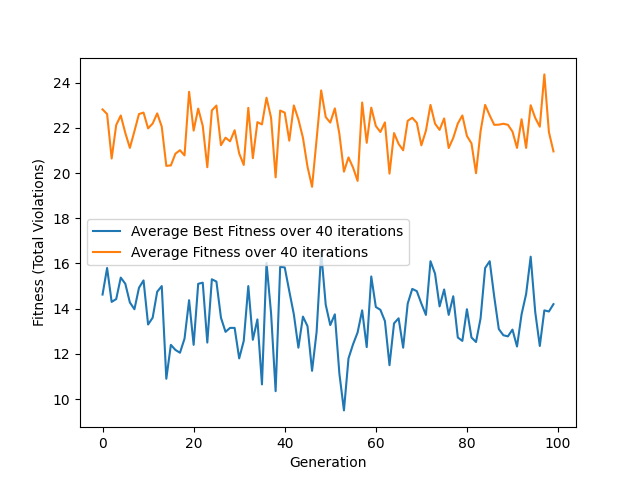
\includegraphics[scale = 0.6]{images/graphcoloring_rb_rd.png}
    \caption {Graph Coloring - RBS \& Random}
    \label {fig:gcRbR}
\end{figure}

\subsection {Overall Analysis}
%FR - 52.26%
%RB - 0.29%
%TT - 0.78%
%RR - 69.9%
%FT - 0.7%
%RT - 0.5%
%TR - 2.2%
%RkR - 47.4%
%RF - 33.15%

\newpage

\section{Final Results}
\subsection{Comparative Analysis}
\begin{table}[ht]
    \centering
    \begin{tabular}{|l|l|l|l|}
    \hline
        \textbf{Parent Selection} & \textbf{Survivor Selection} & \textbf{Best Fitness} & \textbf{Average Fitness} \\ \hline
        \multicolumn{4}{|c|}{\textbf{Knapsack}} \\ \hline
        Fitness Proportion & Random & 982.42 & 645.23 \\ \hline
        Rank Based & Truncation & 1042 & 1039.03 \\ \hline
        Truncation & Truncation & 1037.12 & 1029.05 \\ \hline
        Random & Random & 935.52 & 550.49 \\ \hline
        Fitness Proportion & Truncation & 1037 & 1029.77 \\ \hline
        Random & Truncation & 1037 & 1031.86 \\ \hline
        Truncation & Rank Based & 1042 & 1019.33 \\ \hline
        Rank Based & Random & 1010.95 & 685.83 \\ \hline
        Random & Fitness Proportion & 1008.6 & 757.49 \\ \hline
        \multicolumn{4}{|c|}{\textbf{Graph Coloring}} \\ \hline
        Fitness Proportion & Random & 14.5 & 26.45 \\ \hline
        Rank Based & Truncation & 9 & 10.14 \\ \hline
        Truncation & Truncation & 9 & 9.2 \\ \hline
        Random & Random & 13.45 & 25.24 \\ \hline
        Fitness Proportion & Truncation & 9 & 9.07 \\ \hline
        Rank Based & Fitness Proportion & 14.72 & 25.46 \\ \hline
        Random & Truncation & 7.95 & 8.28 \\ \hline
        Truncation & Rank Based & 7 & 8.43 \\ \hline
        Rank Based & Random & 9.5 & 21.83 \\ \hline
        Random & Fitness Proportion & 17.02 & 30.3 \\ \hline
        \multicolumn{4}{|c|}{\textbf{Travelling Salesman Problem}} \\ \hline
        Fitness Proportion & Random & 65361.51 & 73877.51 \\ \hline
        Rank Based & Truncation & 55745.59 & 56504.16 \\ \hline
        Truncation & Truncation & 59324.92 & 59367.14 \\ \hline
        Random & Random & 65303.59 & 73838.31 \\ \hline
        Fitness Proportion & Truncation & 51655.59 & 52778.71 \\ \hline
        Rank Based & Fitness Proportion & 63406.15 & 72516.23 \\ \hline
        Random & Truncation & 52859.87 & 53402.1 \\ \hline
        Truncation & Rank Based & 51085.47 & 54714.02 \\ \hline
        Rank Based & Random & 63058.26 & 71953.08 \\ \hline
        Random & Fitness Proportion & 65778.02 & 74376.75 \\ \hline
    \end{tabular}
\end{table}

\end{document}